

\documentclass[10pt, titlepage, oneside, a4paper]{article}
\usepackage[T1]{fontenc}
\usepackage[utf8]{inputenc}
\usepackage[swedish]{babel}
\usepackage{amssymb, graphicx, fancyhdr}
\usepackage{hyperref}
\addtolength{\textheight}{20mm}
\addtolength{\voffset}{-5mm}
\renewcommand{\sectionmark}[1]{\markleft{#1}}

\newcommand{\Section}[1]{\section{#1}\vspace{-8pt}}
\newcommand{\Subsection}[1]{\vspace{-4pt}\subsection{#1}\vspace{-8pt}}
\newcommand{\Subsubsection}[1]{\vspace{-4pt}\subsubsection{#1}\vspace{-8pt}}
	


\def\typeofdoc{Laborationsrapport}
\def\course{D0036D}
\def\pretitle{Laboration 3}
\def\title{JavaGameServer \& Client}
\def\name{Magnus Björk}
\def\username{magbjr-3}
\def\email{\username{}@student.ltu.se}
\def\graders{Örjan Tjernström}
\def\university{Luleå Tekniska Universitet}


\def\fullpath{\raisebox{1pt}{$\scriptstyle \sim$}\username/\path}


\begin{document}
	\begin{titlepage}
		\thispagestyle{empty}
		\begin{large}
			\begin{tabular}{@{}p{\textwidth}@{}}
				\textbf{\university \hfill \today} \\
				\textbf{\typeofdoc} \\
			\end{tabular}
		\end{large}
		\vspace{10mm}
		\begin{center}
			\LARGE{\pretitle} \\
			\huge{\textbf{\course}}\\
			\vspace{10mm}
			\LARGE{\title} \\
			\vspace{15mm}
			\begin{large}
				\begin{tabular}{ll}
					\textbf{Namn} & \name \\
					\textbf{E-mail} & \texttt{\email} \\
				\end{tabular}
			\end{large}
			\vfill
			\large{\textbf{Handledare}}\\
			\mbox{\large{\graders}}
		\end{center}
	\end{titlepage}

	\lfoot{\footnotesize{\name, \email}}
	\rfoot{\footnotesize{\today}}
	\lhead{\sc\footnotesize\title}
	\rhead{\nouppercase{\sc\footnotesize\leftmark}}
	\pagestyle{fancy}
	\renewcommand{\headrulewidth}{0.2pt}
	\renewcommand{\footrulewidth}{0.2pt}

	\pagenumbering{roman}
    \tableofcontents
	
	\newpage

	\pagenumbering{arabic}

	\setlength{\parindent}{0pt}
	\setlength{\parskip}{10pt}

	\section{Introduktion}
		Laborationsuppgiften var att programmera ett nätverksspel. Syftet med uppgiften var att man skulle utvidga sin kunskap gällande:
		
        \begin{itemize}
        	\item \textbf{Nätverksprotokoll} 
        		\begin{itemize}
        			\item \textbf{TCP} \\ Pålitligt protokoll för dataöverföring. Lämpligt att använda vid viktiga tillfällen i spelet. \textit{T.ex. när en klient ansluter eller lämnar en server.}
        			\item \textbf{UDP} \\ Opålitligt men snabbt protokoll för dataöverföring. Snabbare än TCP på grund av att det dels inte skickar tillbaka något ACK-meddelande till sändaren samt att UDP har en mindre 'frame'. Lämpar sig bäst för uppdateringar av förflyttningar på grund av sin snabbhet.
        		\end{itemize}
            \item \textbf{Sockets} \\
            Spelet skulle innehålla kommunikation över nätverket, detta sköts av diverse sockets:
            	\begin{itemize}
            		\item \textbf{DatagramSocket} \\Hanterar trafik av protokollet UDP. Kan skicka unicast till en annan DatagramSocket eller multicast genom att skicka till en multicast-grupp. \textit{T.ex. Önskemål om förflyttning från klient till server.}
            		
            		\item \textbf{MulticastSocket} \\Hanterar inkommande multicast-trafik av protokollet UDP. En MulticastSocket går med i en multicast-grupp för att få ta del av dess trafik. \textit{T.ex. uppdateringar av spelarnas position från server till klienter.)}
            		\item \textbf{ServerSocket} \\Serversocket tar emot trafik av protokollet TCP. Ansluter en klient till servern kan man sedan skapa ett Socket objekt för att hantera strömmen.
            		\item \textbf{Socket} \\ Hanterar TCP-trafik. Skapas av ServerSocket på server-sidan. Klienten skapar den socket som tar kontakt med servern.
            		
            	\end{itemize}
          	
			\item \textbf{Trådning} \\En del moment måste köras parallellt och då kan man använda trådar. \textit{T.ex. så har varje klient en tråd på servern som den kommunicerar med.}
        \end{itemize}
        \newpage
        
	\section{Metod}
	
		Min strategi för att lösa uppgiften var att dela upp koden i 3 lager. Detta för att göra det enkelt att lägga på funktioner. \textit{T.ex. Uppgiften att flytta uppdateringsmeddellanden från TCP till UDP var relativt smärtfri, hade spelmekanik varit inblandad i denna del hade det varit betydligt värre.}
		\begin{itemize}
			\item \textbf{Nätverk} Nätverkskoden skall endast skicka meddellanden mellan servern och klienten. Ingenting som har med spel-lagret att göra skall finnas här.
			\item \textbf{Spel} Spelets logik och utseende skall endast påverkas av kommunikations-lagret av programmet.
			\item \textbf{Kommunikation}\\Det lager som sköter kommunikation mellan Spel- och Nätverks-lagren. 
		\end{itemize}
		
		\subsection{Design}
			\begin{center}
				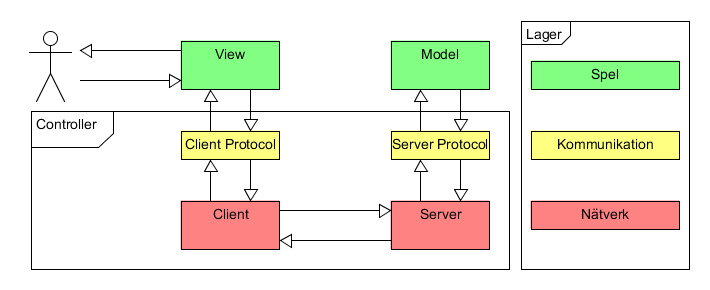
\includegraphics[scale=.5]{./documentation/images/abstract.png}
			\end{center}
			
			Jag ville skapa ett dataflöde liknande bilden ovan.
			\begin{enumerate}
				\item Spelaren trycker på en tangent för att flytta sin markör.
				\item Klient-protokollet skapar ett meddelande med användarens indata och skickar detta till nätverkslagret.
				\item Nätverkslagret skickar nu meddelandet från klienten till servern.
				\item Server-protokollet tar emot och bearbetar modellen efter anvisningar i meddelandet. Skapar ett nytt meddelande som skickas tillbaka till klienten via nätverkslagret.
				\item Klient-protokollet tar emot meddelandet och ändrar eventuellt vyn som visas för spelaren.
				\item Spelaren upptäcker förflyttningen (Om den var giltig) och kan nu ge ny indata om den så vill.
			\end{enumerate}
		
	\section{Resultat}
		\subsection{Användarhandledning}
			\subsubsection{Serverlista}
			När en spelare startar en klient möts denne av denna vy:
				\begin{center}
					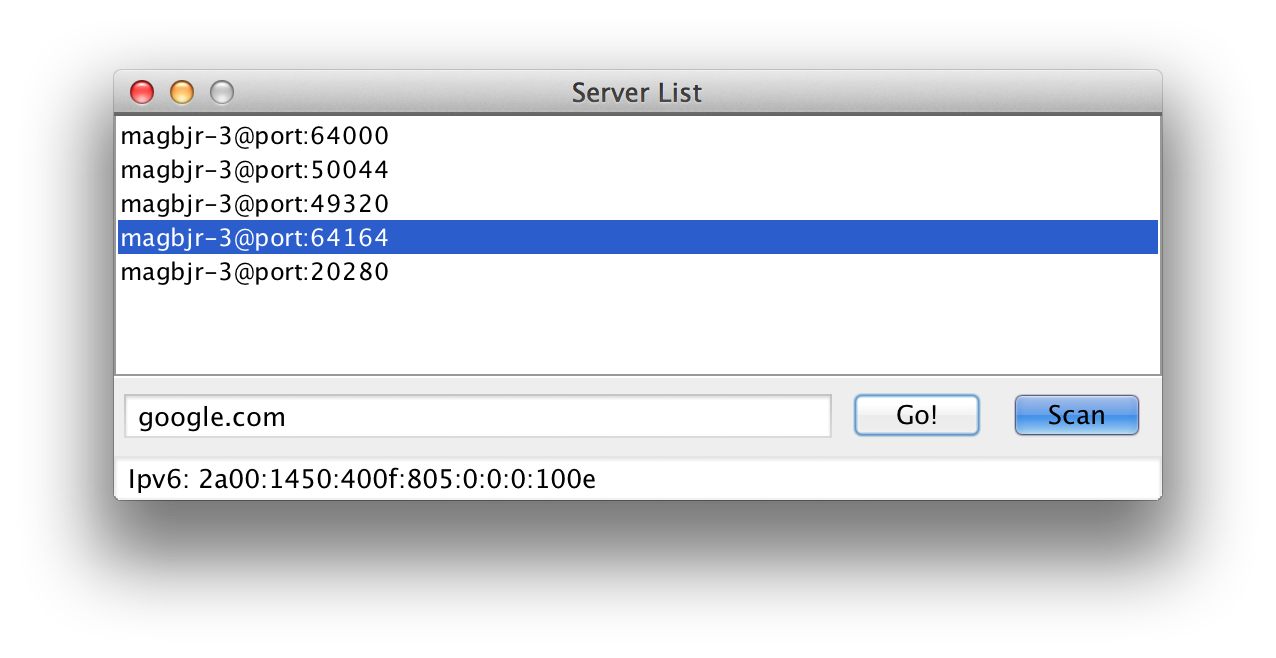
\includegraphics[scale=.5]{./documentation/images/scr2.png}
				\end{center}
				Här kan man användaren göra följande:
				\begin{itemize}
					\item \textbf{Scan}\\Scanna det lokala nätverket efter servrar, hittas en server läggs denne till listan ovan. \textit{Klienten startar 2 trådar, en tråd som skickar ett meddelande till en multicastgroup och en annan tråd som lyssnar efter servrar som svarar på meddelandet. Om en server hittas skickar denne tillbaka en tråd innehållande IP och port nummer. Detta sparas därefter för framtida användande.}
					\item \textbf{Go!}\\I textfältet till vänster om denna knapp kan användaren skriva in en URL. Trycker användaren därefter på knappen 'Go!' så tar programmet reda på IP adressen till denna URL. Finns en Ipv6 adress så är det den som visas. \textit{Programmet använder sig av klassen InetAddress för att ta reda på adressen, sedan används subklassen Inet6Address för att sortera fram Ipv6-adressen.}
					\item \textbf{Serverlista}\\ Har nu användaren hittat sig en server denne vill logga in på så kan användaren göra det genom att dubbel-klicka på en server i listan. \textit{Programmet använder nu IP och port nummer det sparat undan för att kontakta servern via TCP och där startar spelprotokollet.}
				\end{itemize}

			\newpage
			\subsubsection{Spelvy}
			Spelet har nu börjat, om två spelare är inne på samma server kan det se ut så här:
				\begin{center}
					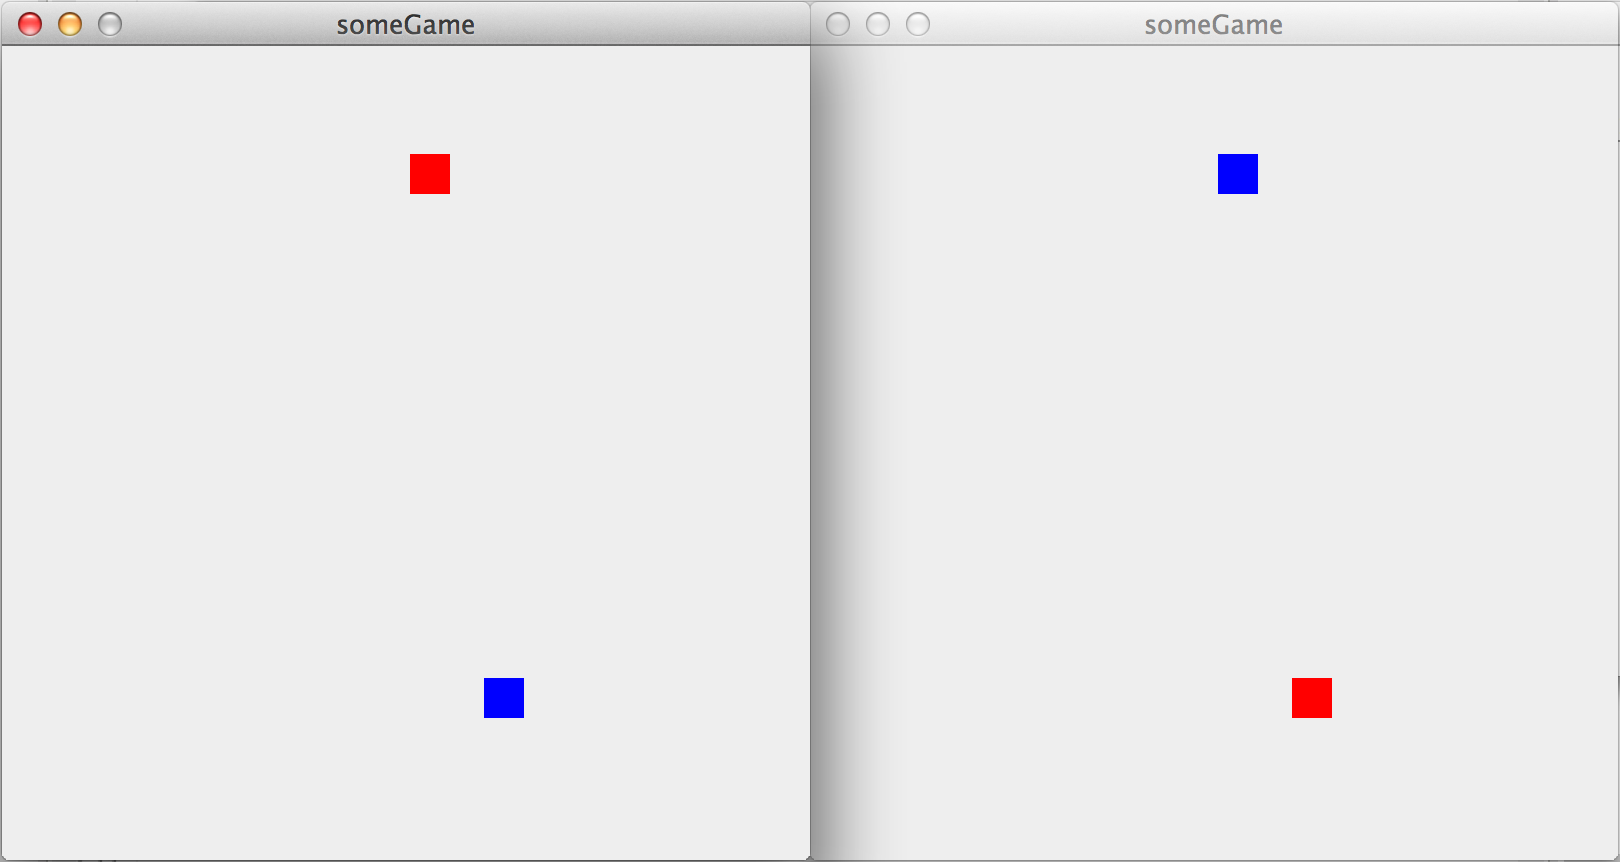
\includegraphics[scale=.3]{./documentation/images/scr1.png}
				\end{center}	
			Röd spelare är den klienten styr, den blå är en annan klient. Objekten kan inte förflytta sig utanför spelplanen,  de kan heller inte förflytta sig 'över' varandra, de kolliderar alltså.\\\\Skulle en spelare vilja avsluta spelet gör denne det genom att stängar ner fönstret, då öppnas föregående fönster igen och spelaren kan antingen välja en annan server eller stänga även detta fönster. Stänger man serverlist fönstret så stängs applikationen.\\\\För de spelare som stannar kvar på servern försvinner helt enkelt den fyrkant som representerade den spelare som lämnade servern.
		
		\subsection{Spelprotokoll}
			\begin{center}
				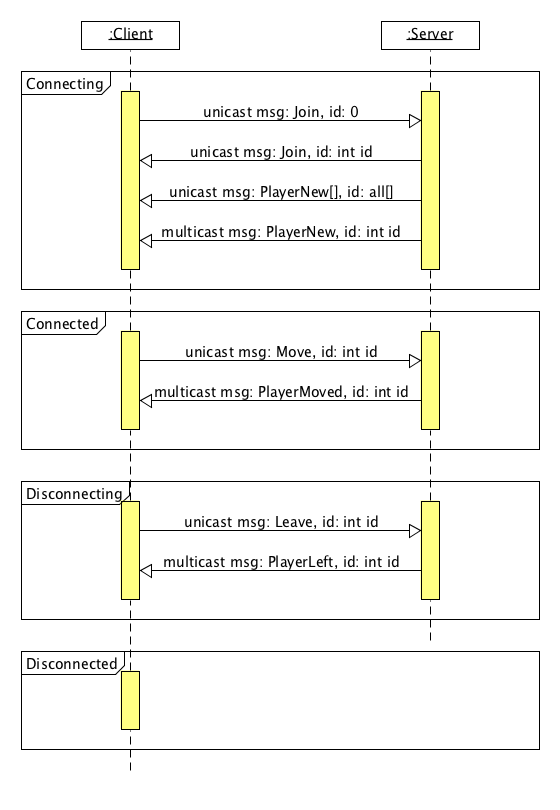
\includegraphics[scale=.5]{./documentation/images/protocol.png}
			\end{center}				
			Klienten har en gameLoop som skapar ett meddelande varje runda. Vilket meddelande som skapas styrs av klientens 4 olika stadier:
				\begin{itemize}
					\item \textbf{Connecting}
						\begin{enumerate}
							\item Klienten har id=0 och skickar meddelande \textit{Join} till servern.
							\item Servern svarar med meddelande \textit{Join} och ger klienten även ett id: \textit{'ID'}.
							\item Servern skickar alla nuvarande spelares position och id till den nya klienten: Meddelande \textit{PlayerNew}.
							\item Servern skickar den nya spelarens position till alla spelare på servern, även den nya spelaren: Meddelande \textit{PlayerNew}.
							\item \textbf{När klienten upptäcker att den nya spelaren är sig själv (\textit{'ID'}) byter klienten stadium till 'Connected'.}
						\end{enumerate}
						
					\newpage
					\item \textbf{Connected}
						\begin{enumerate}
							\item Nu kollar klienten om spelaren gett input via tangentbordet, har denne gjort det skapas ett meddelande: \textit{Move} med riktning av förflyttningen samt klientens \textit{'ID'}. Detta skickas till servern via UDP.
							\item Servern tar emot datagrammet från klienten och undersöker om förflyttningen är giltig. Är den det skickas meddelandet: \textit{PlayerMoved} med \textit{'ID'} till samtliga klienter via UDP multicastsocket. Annars skickas ingenting.
							\item Klienten tar emot meddelandet och ritar ut förflyttningen på spelplanen.
							\item \textbf{Detta pågår tills dess att spelaren stänger ner spelfönstret, då sätts klientens stadium till 'Disconnecting'.}
						\end{enumerate}
					\item \textbf{Disconnecting}
						\begin{enumerate}
							\item Klienten skickar nu ett meddelande: \textit{Leave} till servern.
							\item Servern raderar alla spår av klienten i modellen och skickar meddelandet: \textit{PlayerLeft} till alla klienter.
							\item Klienten upptäcker att den har lämnat server genom att \textit{'ID'} stämmer överens med sitt eget id.
							\item \textbf{Klienten sätter sitt stadium till 'Disconnected'.}
						\end{enumerate}
					\item \textbf{Disconnected}\\I detta stadium har finns inte någon koppling mellan servern och klienten. Klienten avslutar nu sina trådar och applikationen startar serverlistvyn igen.
				\end{itemize}
				
		\newpage
		\subsection{Trådar}
			\begin{center}
				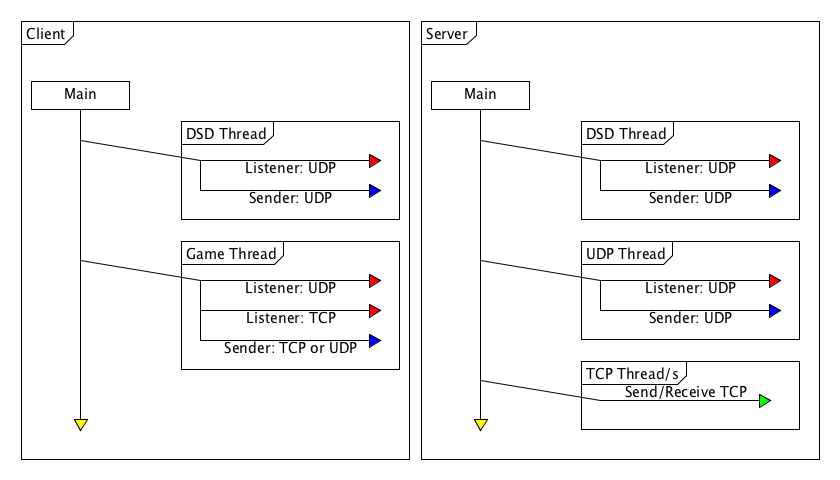
\includegraphics[scale=.4]{./documentation/images/threads.png}
			\end{center}
			\subsubsection{Klient}
				Klienten startar har följande trådar:
				\begin{itemize}
					\item \textbf{DSD: Dynamic Service Discovery}\\ Används för att hitta spelservrar genom att skicka strängen SERVICE QUERY JavaGameServer till en muticast-grupp. Sänder ut denna sträng medans knappen "Scan" är intryckt. Startar även tråd:
					\begin{itemize}
						\item UDP lyssnar tråd. Denna tråd tar emot svar från hittade servrar.
					\end{itemize}
					
					\item \textbf{Game Thread}\\Den tråd spelet körs i. TCP/UDP-ut körs även här. Detta för att endast ett meddelande kommer att gå ut från klienten per cykel av klientens gameLoop. Startar ytterligare två trådar:
						\begin{itemize}
							\item TCP lyssnar tråd. För att inte blocka multicast över TCP från server trådar så har klienten en egen tråd för TCP in.
							\item UDP lyssnar tråd. För att inte blocka klienten så har även UDP-in en egen tråd.
							
						\end{itemize}
				\end{itemize}
			\newpage
			\subsubsection{Server}
				Serverns antal trådar beror på antal klienter anslutna. Trådarna är:
				\begin{itemize}
					\item \textbf{DSD Thread}\\Börjar med att lyssna efter klienter som vill hitta servern. Tar en klient kontakt med servern skickas serverns IP och port nummer tillbaka till klienten. Startas vid serverstart, \textbf{en tråd per server}.
					\item \textbf{UDP Thread}\\Lyssnar efter förflyttnings-förfrågningar av klienter, skickar tillbaka förflyttning till alla klienter kopplade till servern om förflyttning beviljas. Startas i sammband med serverstart, \textbf{en tråd per server} krävs.
					\item \textbf{TCP Thread}\\Sänder och tar emot meddellanden som skickas till servern över TCP. Startas när en klient ansluter till servern, därför krävs \textbf{en tråd per ansluten klient}.
				\end{itemize}
	
	\newpage
	\section{Diskussion}
		Laborationen var intressant och givande. Det hade dock varit kul om det hade varit krav på att spelet skulle följa ett specifikt protokoll likt laboration 4. Detta för att kunna testa servrarna/klienterna mot sina klasskamraters.\\\\
		\textbf{Datagram*/Packet/Socket}\\Efter att ha arbetat med TCP strömmar tog det ett tag att ställa om tankesättet till UDP. Men om man tänker DatagramSocket som en brevlåda, DatagramPacket som ett kuvert och Datagram som ett brev så blir det lite klarare. Man skulle kunna tänka sig att man sätter ett tomt kuvert i sin brevlåda och väntar på att en brevbärare stoppar in ett brev i kuvertet, när han gjort det målar han om brevlådan och då vet man att det finns ett brev inuti kuvertet!
		
		\subsection{Lösningens begränsningar} 
		\subsubsection{Objekt} Strukuren på programmet såg bra ut till en början, men ju fler funktioner som lagts till desto grötigare har koden blivit. 
		\subsubsection{Synchronize} Kollisionsdetektionen är inte synkroniserad. Detta gör att om flera spelare spelar samtidigt finns möjligheten att deras objekt fastnar i varandra. Detta problem kan man lösa lätt genom att sätta 'synchronize' på metoden som utför kollionskollen.
		\subsubsection{Instabilitet} Om klienten försöker ansluta till en server som svarar med samma DSD sträng men inte följer samma spelprotokoll så kraschar den. Även server är känslig för klienter som ansluter med samma DSD sträng men annat protokoll.
		\subsubsection{Threadpool} Servern startar en tråd för varje anslutning, därför blir servern öppen för DoS(Denial of Service) attacker. Detta hade man kunnat lösa genom att skapa en threadpool (Servern får bara använda ett givet antal trådar.).
    
    
\end{document}
